\chapter{Results}
\label{chap:results}

This chapter covers the results and interpretation of the fitting procedure described in the previous chapter, including the upper limits on signal yields for the \ttDM process in the dilepton channel presented in Section~\ref{sec:UL}. Section~\ref{sec:comparetoDD} presents the results in the same planes as results from direct and indirect dark matter detection experiments. 

\section{Simplified model interpretation}
\label{sec:interpretation}
Dark matter production at colliders can be characterized, in large part, by the interaction between the SM and DM particles. The main characteristics of the simplified models under consideration are briefly highlighted in Sec.~\ref{sec:simpmodels}, and will be expanded upon in the following section.

Prior to Run II of the LHC, DM searches such as the one detailed in~\cite{Khachatryan:2016reg}, had been traditionally interpreted using Effective Field Theory (EFT) models~\cite{Goodman:2010ku}, wherein the interaction between the SM particles and the Dirac fermion WIMPs is mediated through higher dimensional operators. The models are solely characterized by the DM mass, \mDM, and $M_{*}$ which represents the strength of the interaction and is a function of the masses and coupling strengths of the mediating particles between the DM and SM fields. The benefits of the EFT formulation is the lack of model dependence, and the relative ease encountered in translating experimental collider constraints to the direct detection DM-nucleon cross section-\mDM plane. The shortcoming of such field theories, however, are that they are non-renormalizable, thus they become invalid at arbitrarily high energy scales, and this is represented by the masses of the mediating particles that have been integrated out. In general, for an EFT to make sense, it is required that $M_{*}$ must be much larger than the energy transfer through quarks at the LHC, i.e. $M_{*}^{2} >> Q_{\textrm{tr}}^{2}$. Thus, since this class of models does not truly account for the mediator, effects from resonant enhancement are not included and EFTs have no sensitivity to off-shell mediator production.

\begin{figure}
  \subfloat[][]{\label{fig:EFT}
    \feynmandiagram[vertical=b to d]{
      a [particle=\(\bar{t}\)] -- [fermion] b -- [fermion] c -- [fermion] d -- [fermion] e [particle=\(t\)],
      f [particle=\(g\)] -- [gluon] b,
      g [particle=\(g\)] -- [gluon] d,
      h [particle=\(\bar{\chi}\)] -- [fermion] c -- [fermion] i [particle=\(\chi\)],
      h -- [opacity=0.001] i,
      %%f -- [opacity=0.001] g,
      a -- [opacity=0.001] h,
      e -- [opacity=0.001] i,
    };
  }
  \hspace{0.5cm}
  \subfloat[][]{\label{fig:DMF}
    \feynmandiagram[horizontal=c to h]{
      a [particle=\(\bar{t}\)] -- [fermion] b -- [fermion] c -- [fermion] d -- [fermion] e [particle=\(t\)],
      f [particle=\(g\)] -- [gluon] b,
      g [particle=\(g\)] -- [gluon] d,
      c -- [scalar, edge label=\(\phi \slash a\)] h,
      i [particle=\(\bar{\chi}\)] -- [fermion] h -- [fermion] j [particle=\(\chi\)],
      e -- [opacity=0.0001] i,
      a -- [opacity=0.0001] j,
      i -- [opacity=0.0001] j,
      %%      f -- [opacity=0.0001] g,
    };
  }
  \caption{The representative diagram of a top quark pair produced in association with a pair of DM particles ($\chi\bar{\chi}$) using~\protect\subref{fig:EFT} the EFT formalism and~\protect\subref{fig:DMF} the simplified model formalism.}
\end{figure}

In order to circumvent the deficiencies of the EFT formalism, a class of simplified models have been employed for the interpretation of DM searches during Run II of the LHC. In part, the increase in the center-of-mass collision energy from $\sqrt{s}=8\:\TeV$ to $\sqrt{s}=13\:\TeV$ limits the region of validity for the EFT models. Hence, the contact interaction of the EFT models, as depicted in~\FigureRef{fig:EFT} is subsequently resolved into a mediator interaction which couples to the SM and DM particles, as shown in~\FigureRef{fig:DMF}. 

The interaction Lagrangians of the scalar ($\phi$) and pseudoscalar ($a$) mediators are as follows~\cite{Abercrombie:2015wmb},

\begin{equation}
  \mathcal{L}_{\phi} = g_{\chi}\phi\chi\bar{\chi} + \frac{\phi}{\sqrt{2}}\sum_{i}{(g_{u}y_{i}^{u}\bar{u}_{i}u_{i} + g_{d}y_{i}^{d}\bar{d}_{i}d_{i} + g_{\ell}y_{i}^{\ell}\bar{\ell}_{i}\ell_{i})},\\
  \mathcal{L}_{a} = ig_{\chi}a\chi\gamma_{5}\bar{\chi} + \frac{ia}{\sqrt{2}}\sum_{i}{(g_{u}y_{i}^{u}\bar{u}_{i}\gamma_{5}u_{i} + g_{d}y_{i}^{d}\bar{d}_{i}\gamma_{5}d_{i} + g_{\ell}y_{i}^{\ell}\bar{\ell}_{i}\gamma_{5}\ell_{i})}
\end{equation}

where the Yukawa couplings are $y_{i}^{f} = \sqrt{2}m_{i}^{f}/v$, where $m^{f}_{i}$ is the fermion mass, and $v=246\:\GeV$ is the Higgs boson field vacuum expectation value. $g_{\chi}, g_{u}, g_{d}$ and $g_{\ell}$ represent the coupling strength between the mediator and the dark sector, up-type quarks, down-type quarks, and leptons respectively. In the report issued by the Dark Matter Forum (DMF)~\cite{Abercrombie:2015wmb}, a collaboration between members of CMS, ATLAS and the theory community, a benchmark set of parameters for the relevant simplified models of DM were chosen after scans of the parameter space were performed. In the following analysis, the DMF recommendation of $g_{\chi} = g_{u} = g_{d} = g_{\ell} = 1$ is followed. This reduces the free parameters to \{\mDM, \mMed\} which contribute to the minimal mediator width at LO via, 

\begin{equation}
  \Gamma_{\phi} = \frac{\mDM}{8\pi}\Big(1-\frac{4\mDM^{2}}{m_{\phi}^2}\Big)^{x/2} + \sum_{f=fermions}\frac{y_{f}^{2}m_\phi}{16\pi}\Big(1 - \frac{4m_{f}^2}{m_{\phi}^2}\Big)^{x/2},
\end{equation}

with $x=3$ for scalar mediators, and $x=1$ for pseudoscalar mediators. Owing to the choice of SM Higgs-like Yukawa couplings for the SM fermions, the top quark contribution to the mediator width is enhanced at mediator masses above twice the top quark mass, but conversely for lighter mediator masses, the DM contribution dominates since couplings to the lighter quarks are Yukawa-suppressed. Thus the sensitivity of this search is concentrated in the low mediator mass regime, below twice the top quark mass. The signal samples used in the analysis were generated at LO accuracy in QCD with up to one additional parton in the final state, however as described in Ref.~\cite{Backovic:2015soa}, the cross section is computed at NLO with no additional partons in the Born process, and the samples are normalized to the NLO values listed in Table~\ref{tab:NLOxsec}

\begin{table}
  \centering
  \begin{tabular}{|r|r|c|c|}
    \hline
    \mMed [GeV] & \mDM [GeV] & Scalar (pb) & Pseudoscalar (pb) \\
    \hline
    %% NLO %%
    10  & 1 & $26.09   $ & $0.6218$  \\
    20  & 1 & $13.96   $ & $0.5653$  \\
    50  & 1 & $3.923   $ & $0.4314$  \\
    100 & 1 & $0.8891  $ & $0.2716$  \\
    200 & 1 & $0.1229  $ & $0.1189$ \\
    300 & 1 & $0.04079 $ & $0.05946$ \\
    500 & 1 & $0.007796$ & $0.008171$\\
    \hline
  \end{tabular}
  \caption{Summary of the signal samples and the correpsonding NLO cross sections used in this analysis for scalar and pseudoscalar mediator masses with $\mDM=1\:\GeV$.}
  \label{tab:NLOxsec}
\end{table}

\section{Upper limits on \ttDM production in the dilepton channel}
\label{sec:UL}

From the background-only post-fit yields presented in Table~\ref{tab:cat-hi_postfit_yields} and~\ref{tab:cat-lo_postfit_yields}, it is apparent that there is no significant excess of events expected over the SM backgrounds, hence $95\%$ $\textrm{CL}_{s}$ upper limits on the signal strength parameter $\mu$ defined in Section~\ref{subsec:signal} are set. The expected and observed upper limits on $\mu$ for signal models with varying scalar and pseudoscalar mediator masses and $\mDM=1\:\GeV$ are listed in Table~\ref{tab:results} along with the $\pm\:1\sigma$ and $\pm\:2\sigma$ uncertainties on the expected limit. The results shown in the tables are visualized in~\FigureRef{fig:scalar_results} and~\FigureRef{fig:pseudo_results} as a function of \mMed, where the couplings are assumed to be \gq = \gDM = 1 and the DM mass is \mDM = 1 \GeV. The range of \mMed are deemed as excluded by the search, when the upper limit on $\mu$ is less than 1. As can be seen in~\FigureRef{fig:scalar_results} and~\FigureRef{fig:pseudo_results}, the observed (expected) $95\%$ $\textrm{CL}_{s}$ exclusions for a scalar mediator are $\mMed<74(99)\:\GeV$, while for a pseudoscalar mediator, the expected exclusion is $m_{a}<50\:\GeV$, and no exclusion is observed. 

\begin{table}
  \begin{tabular}{|l|c|c|c|c|}
    \hline
    Model (\mMed,\mDM) [GeV] &   Obs.  &    Exp. &  $[  -1\sigma, +1\sigma  ]$ &  $[  -2\sigma, +2\sigma  ]$ \\ \hline
    S  10,   1 &      0.72 &     0.59 &   $[   0.41,    0.89]$ &  $[   0.30,    1.32]$ \\
    S  20,   1 &      0.64 &     0.51 &   $[   0.35,    0.76]$ &  $[   0.25,    1.11]$ \\
    S  50,   1 &      0.74 &     0.62 &   $[   0.43,    0.94]$ &  $[   0.31,    1.36]$ \\
    S 100,   1 &      1.29 &     1.01 &   $[   0.69,    1.51]$ &  $[   0.51,    2.19]$ \\
    S 200,   1 &      2.97 &     2.40 &   $[   1.64,    3.58]$ &  $[   1.19,    5.22]$ \\
    S 300,   1 &      5.64 &     4.61 &   $[   3.16,    6.91]$ &  $[   2.30,   10.11]$ \\
    S 500,   1 &     22.93 &    18.74 &   $[  12.78,   28.52]$ &  $[   9.26,   42.20]$ \\ 
    \hline
    PS  10,   1 &      1.16 &     0.92 &   $[   0.63,    1.38]$ &  $[   0.46,    2.01]$ \\
    PS  20,   1 &      1.16 &     0.92 &   $[   0.63,    1.38]$ &  $[   0.46,    2.01]$ \\
    PS  50,   1 &      1.26 &     1.00 &   $[   0.69,    1.50]$ &  $[   0.50,    2.19]$ \\
    PS 100,   1 &      1.49 &     1.18 &   $[   0.81,    1.77]$ &  $[   0.59,    2.59]$ \\
    PS 200,   1 &      2.45 &     1.95 &   $[   1.33,    2.93]$ &  $[   0.96,    4.30]$ \\
    PS 300,   1 &      3.99 &     3.23 &   $[   2.19,    4.89]$ &  $[   1.60,    7.22]$ \\
    PS 500,   1 &     22.29 &    18.06 &   $[  12.15,   27.49]$ &  $[   8.78,   41.31]$ \\\hline
  \end{tabular}
  \caption{Observed and expected upper limits at $95\%$ $\textrm{CL}_{s}$ on $\mu$ as a function of scalar (S) and pseudoscalar (PS) mediator masses for $\mDM=1\:\GeV$ with $\pm\:1\sigma$ and $\pm\:2\sigma$ uncertainties on the expected limits.}
  \label{tab:results}
\end{table}

\begin{figure}
  \centering
  \subfloat[][Upper limits for scalar mediators]{
    \label{fig:scalar_results}
    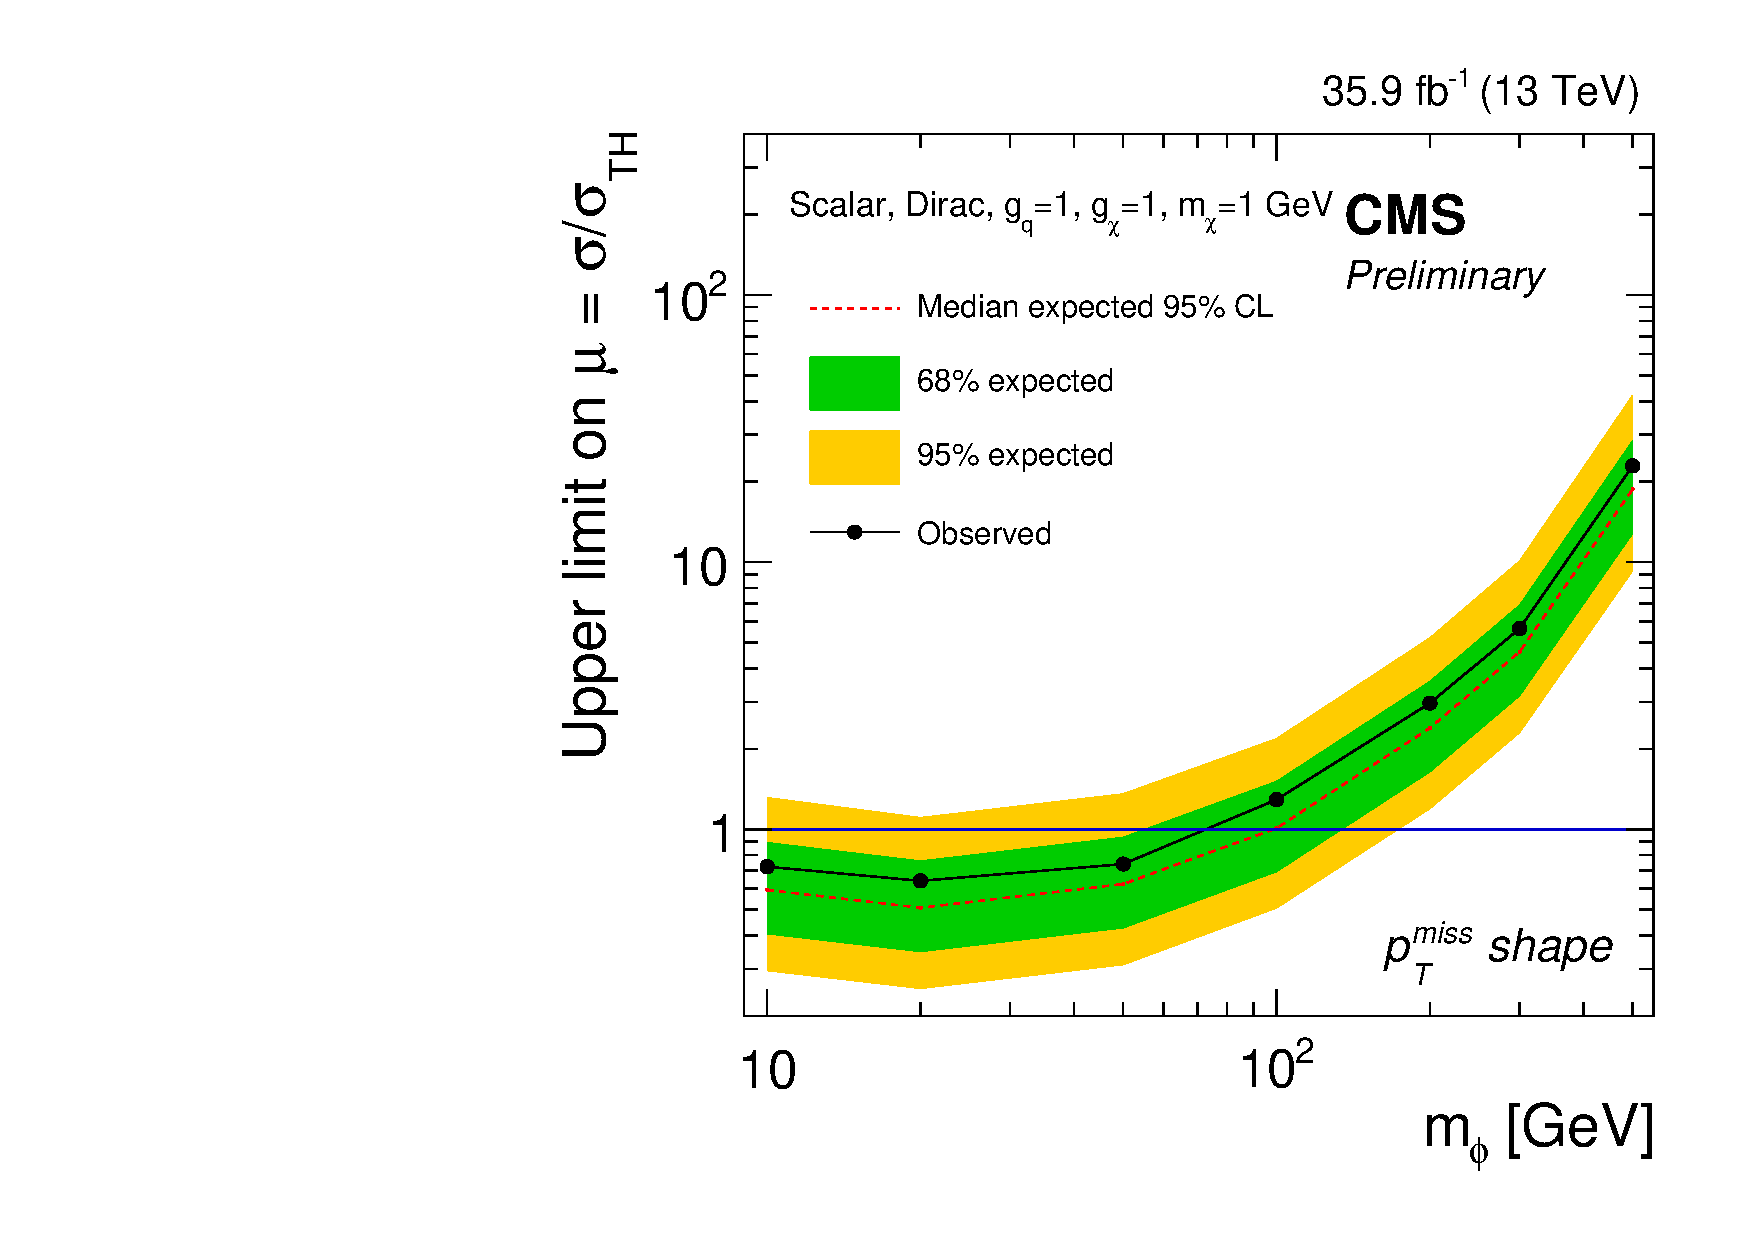
\includegraphics[width=0.6\textwidth]{figs/dilepton_S_NLO_limits.pdf}
  } 
  \hspace{1 cm}
  \subfloat[][Upper limits for pseudoscalar mediators]{
    \label{fig:pseudo_results}
    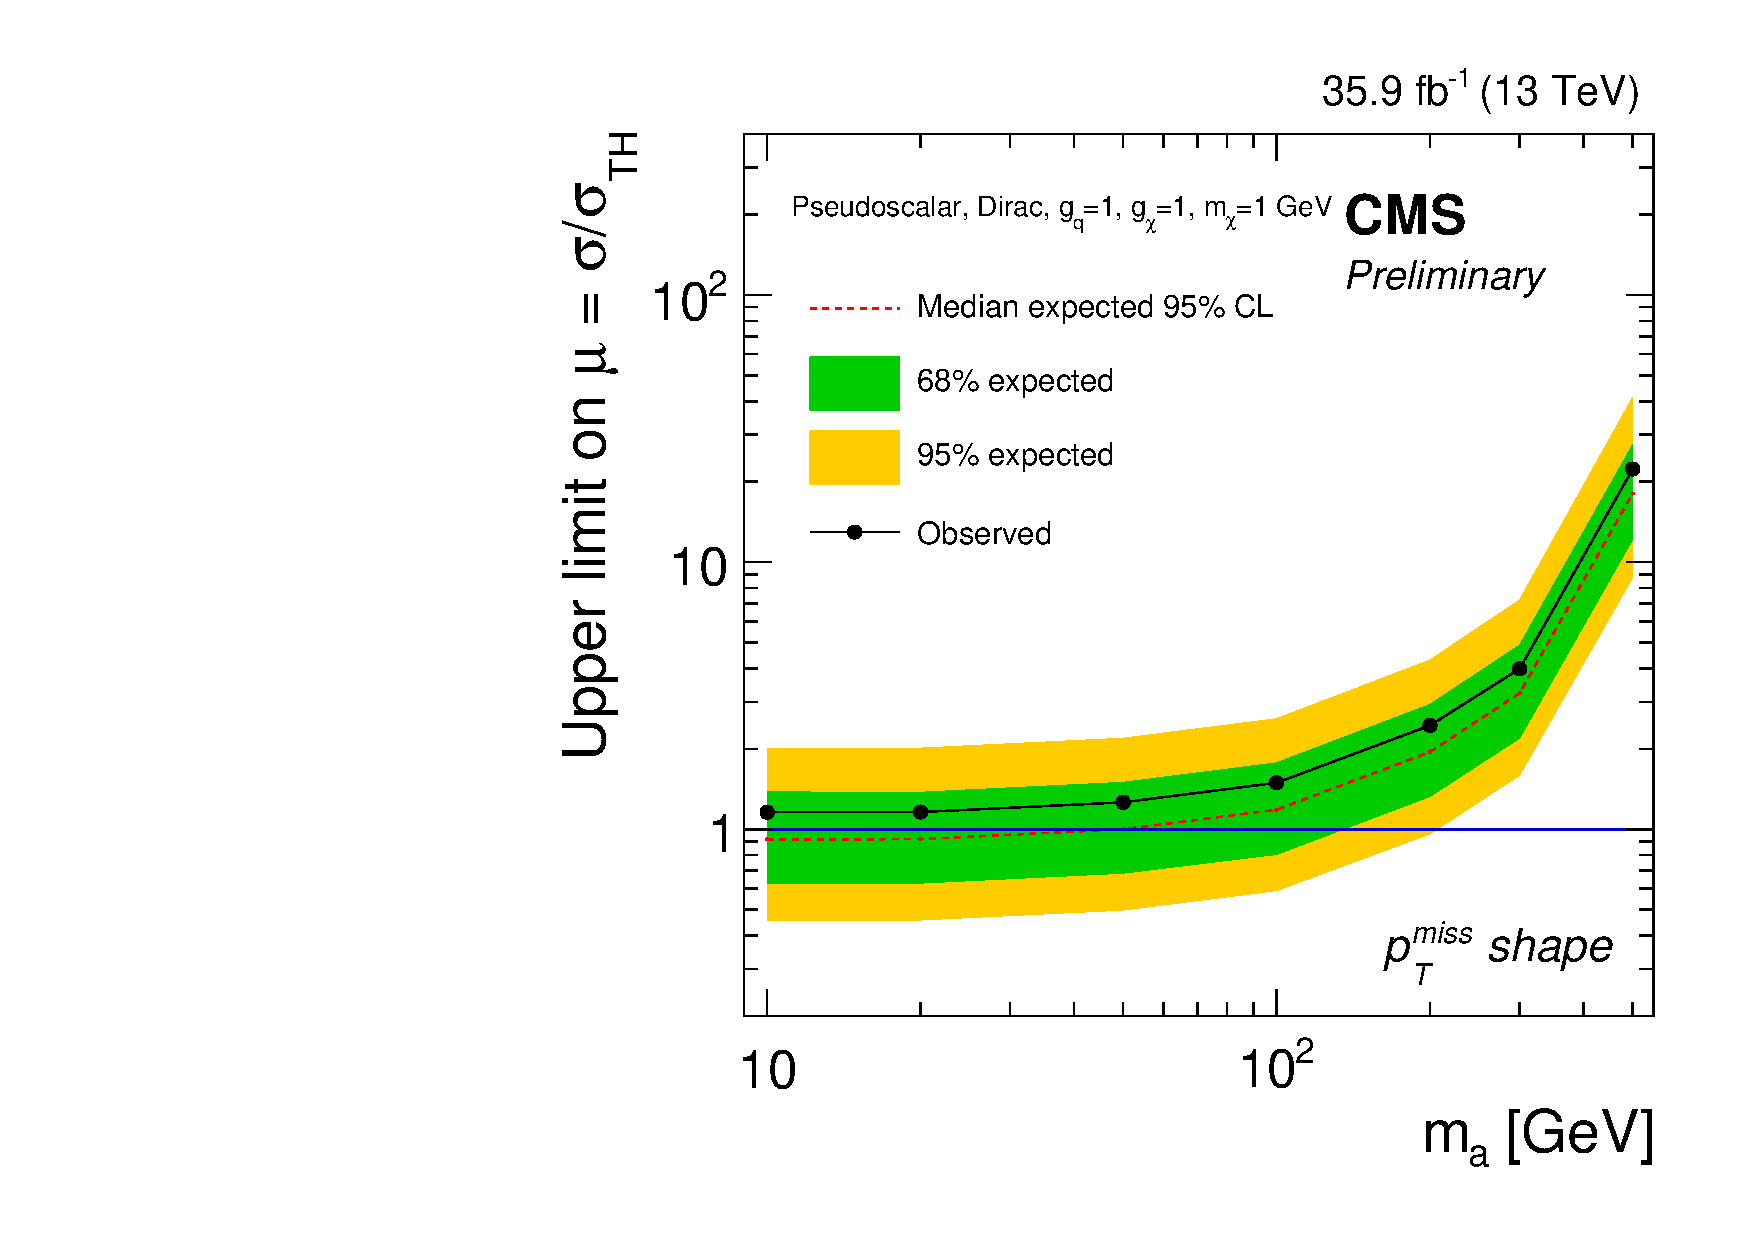
\includegraphics[width=0.6\textwidth]{figs/dilepton_PS_NLO_limits.pdf}
  }
  \caption{The expected (red dashed) and observed (solid black) $95\%$ $\textrm{CL}_{s}$ upper limits on the \ttDM signal strength in the dilepton channel for various~\protect\subref{fig:scalar_results} scalar and~\protect\subref{fig:pseudo_results} pseudoscalar mediator masses where $\mDM=1\:\GeV$ and $\gq = \gDM = 1$ is assumed. The results are obtained using $35.9\:\textrm{fb}^{-1}$ collected by the CMS detector in 2016.}
\end{figure}

The upper limits for on the scalar mediated \ttDM signal are also shown as a function of \mMed and \mDM in~\FigureRef{fig:2Dexclusion}. The solid (finely dashed) contour encloses the region where the observed (expected) upper limit on $\mu$ is less than 1. It should be noted that the narrow width of the mediator causes the cross section to drop off very rapidly across the on-/off-shell (\mMed = 2\mDM) line, therefore the exclusion contour runs close to the diagonal but does not cross it.

\begin{figure}
  \centering
  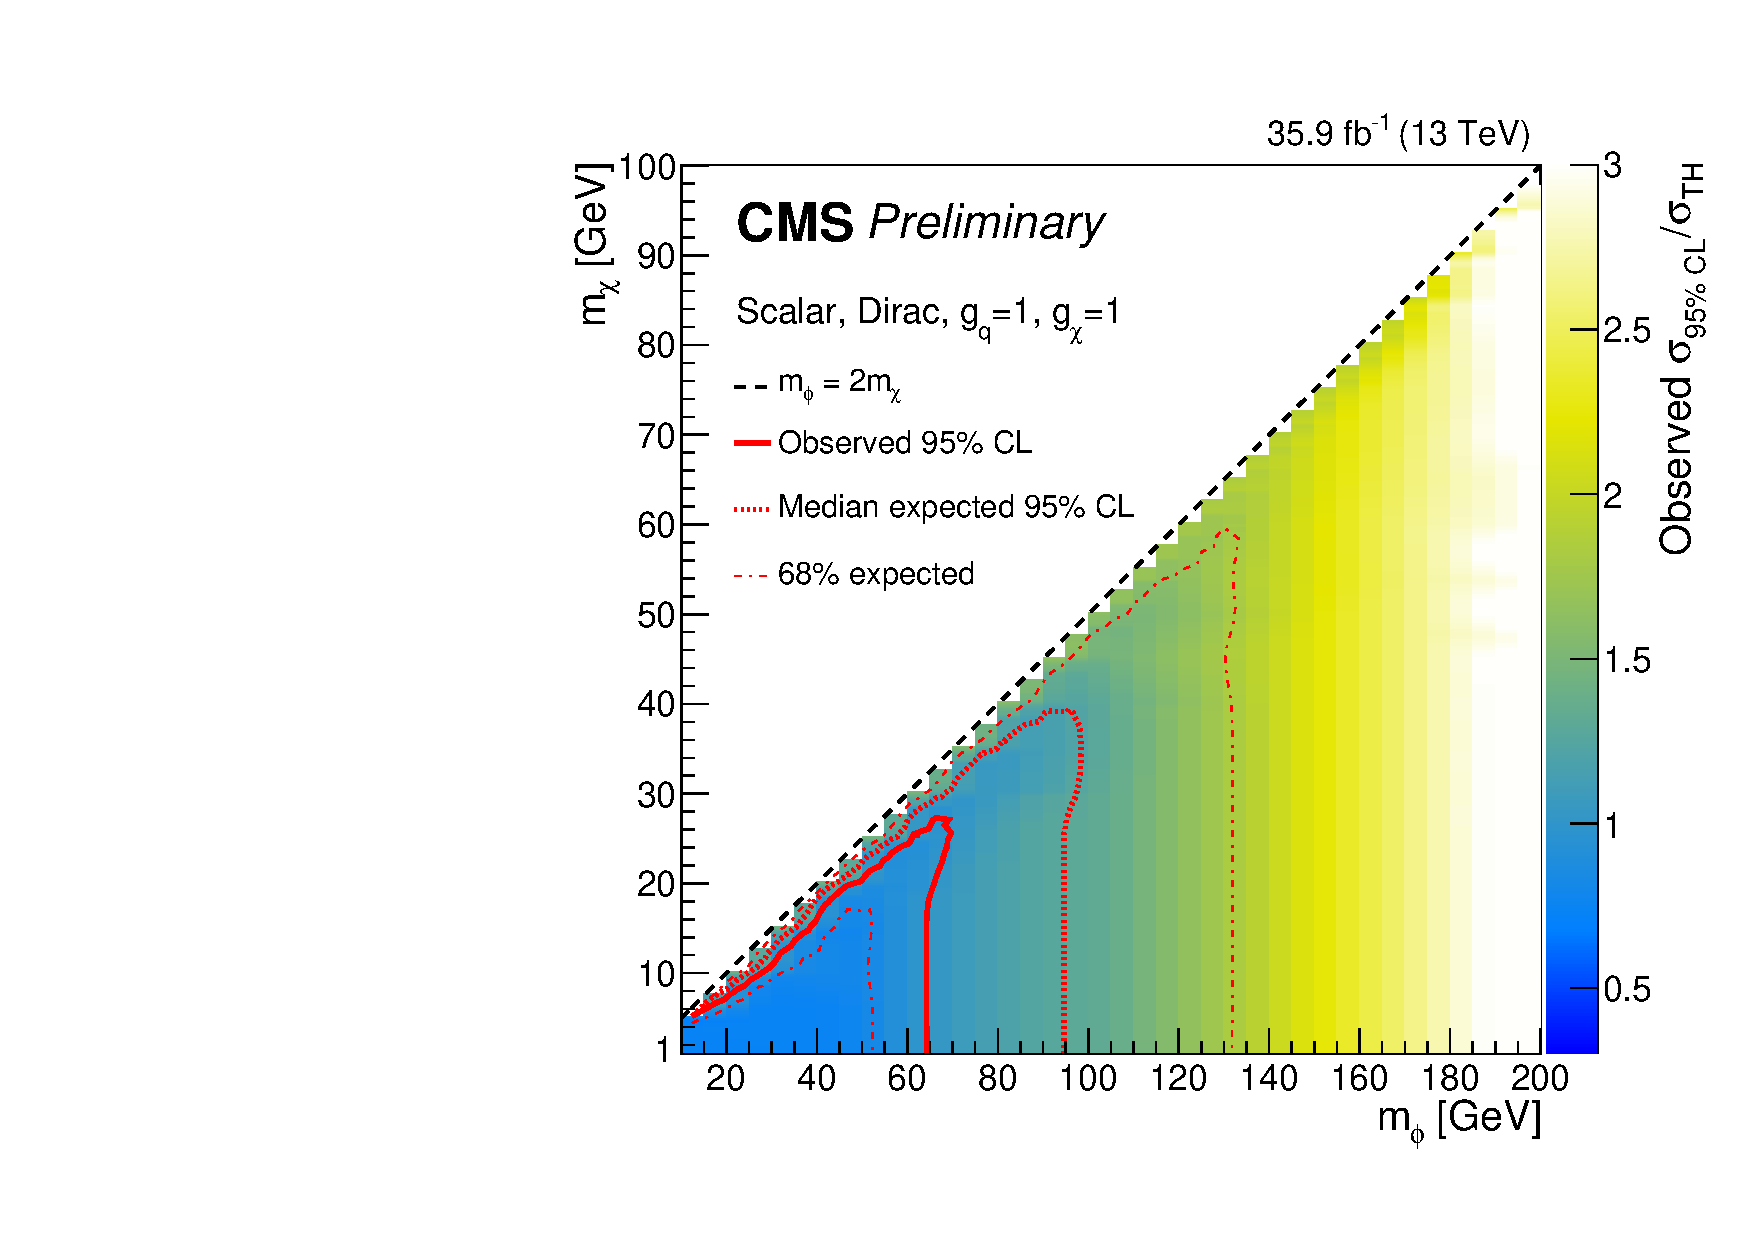
\includegraphics[width=0.65\textwidth]{figs/dilept_inc_S_limits2D_NLO.pdf}
  \caption{The exclusion limits at $95\%$ $\textrm{CL}_{s}$ on the signal strength parameter $\mu$ for the \ttDM process in the dilepton channel, computed as a function of the mediator mass and DM mass, assuming a scalar mediator. The mediator couplings are assumed to be $\gq=\gDM=1$.}
  \label{fig:2Dexclusion}
\end{figure}

\clearpage 

\section{Comparison with direct detection}
\label{sec:comparetoDD}

To facilitate the comparison with constraints from direct detection experiments, the exclusion contours obtained from the scalar \ttDM model as shown in~\FigureRef{fig:2Dexclusion} are calculated at $90\%$ $\textrm{CL}_{s}$. Subsequently, the upper limits on $\mu$ are translated to upper limits on the spin-independent (SI) DM-nucleon scattering cross section via the approach taken from Ref.~\cite{Boveia:2016mrp} as briefly described in the proceeding section.

\subsection{Spin-indepedent comparison}
\label{subsec:SIcase}

The general form of the spin-independent DM-nucleon scattering cross section is,

\begin{equation}
  \sigma_{\textrm{SI}} = \frac{f^{2}(\gq)\gDM^{2}\mu_{n\chi}^2}{\pi\mMed^{4}}
  \label{eq:DDtranslation}
\end{equation}

where $\mu_{n\chi} = m_{n}\mDM/(m_{n}+\mDM)$ is the DM-nucleon reduced mass with $m_{n} \simeq 0.939\:\GeV$ being the approximate nucleon mass. The mediator-nucleon coupling, denoted by $f(\gq)$, has a non-trivial dependence on the mediator-quark couplings and the Higgs boson vacuum expectation value, so the full definition is ommitted. However, using the most state-of-the-art values for these dependencies from Refs.~\cite{Hoferichter:2015dsa} and~\cite{Junnarkar:2013ac}, the numerical value of $f(\gq)$ is,

\begin{equation}
  f(\gq) = 1.16 \times 10^{-3} \gq.
\end{equation} 

Thus, Eq.~\ref{eq:DDtranslation} takes the form,

\begin{equation}
  \sigma_{\textrm{SI}} \simeq 6.9 \times 10^{-43} \Big(\frac{\gq\gDM}{1}\Big)^{2}\Big(\frac{125\:\GeV}{\mMed}\Big)^{4}\Big(\frac{\mu_{n\chi}}{1\:\GeV}\Big)^{2}.
\end{equation}

As a result, the upper limit on $\mu$ for the scalar-mediated \ttDM process in the dilepton channel is presented as a bound in the \mDM-$\sigma_{\textrm{SI}}$ plane in~\FigureRef{fig:DDplot}. The assumptions made in the translation include that the DM particle is a Dirac fermion, the coupling values are $\gq = \gDM = 1$, and the CMS expected and observed exclusions are calculated at $90\%$ $\textrm{CL}_{s}$, as is standard in the direct detection community. The collider limits are the most constraining at low DM mass, which is well-supported by the strong constraints at low \mMed as seen in the limit curve in~\FigureRef{fig:scalar_results} where \mDM=1 \GeV.

\begin{figure}
  \centering
  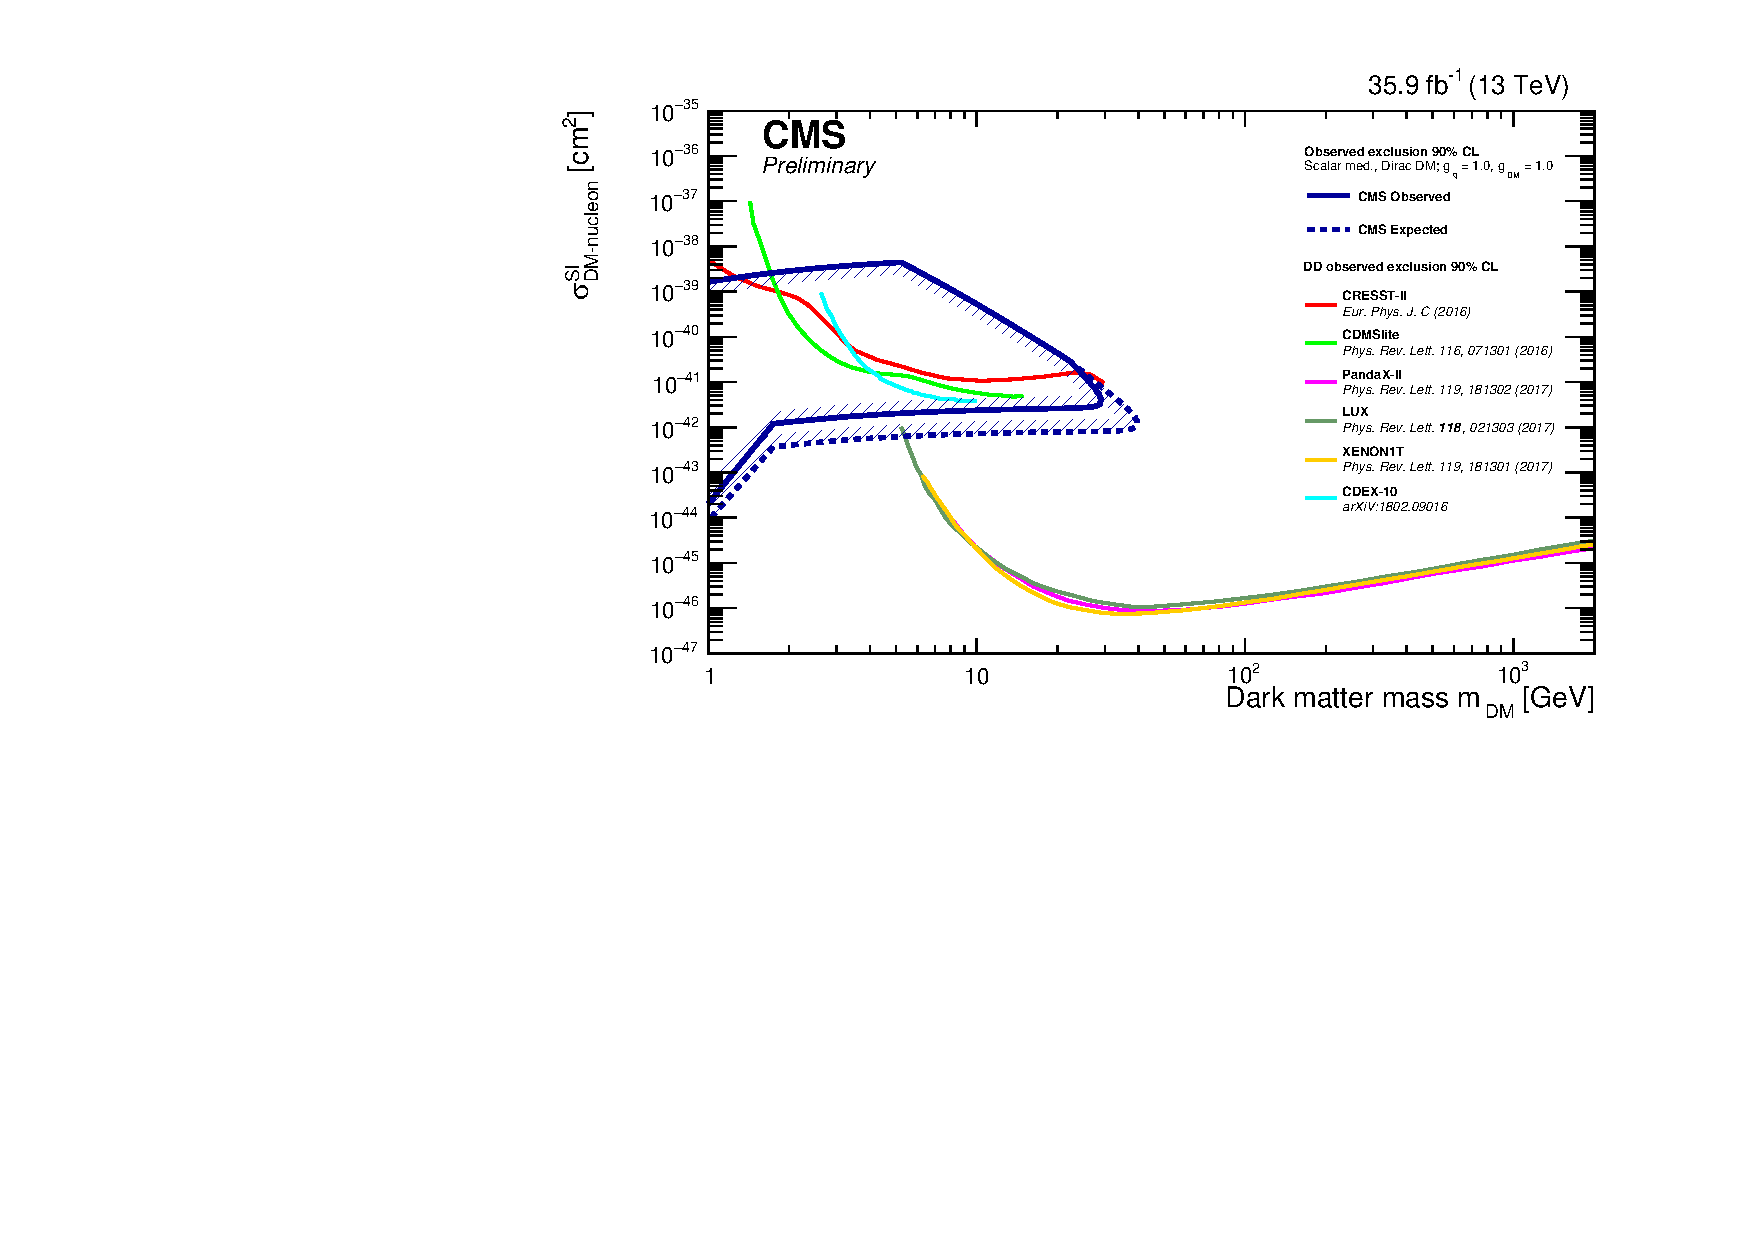
\includegraphics[width=\textwidth]{figs/SIS_CMSDD_Summary.pdf}
  \caption{A comparison of the \ttDM scalar-mediated results in the dilepton channel (CMS expected and observed lines) to the exclusion contours of the LUX, PandaX-II, XENON1T, CDEX-10, CDMSLite, and CRESST-II limits in the \mDM-$\sigma_{\textrm{SI}}$ plane. The DM particle is assumed to be a Dirac fermion and $\gq = \gDM =1$.}
  \label{fig:DDplot}
\end{figure}
